\skriptsection{Fourierreihen}{67ff}
    \skriptsubsection{Orthogonalitätsbeziehungen der Basisfunktionen}{75}
        \begin{tabular}{lll}
            $\int\limits_0^T \cos(n\omega t)\cdot \cos(m\omega t)dt=
            \begin{cases}
            T,\ n=m=0\\
            \frac{T}{2},\ n=m>0\\ 
            0,\ n\neq m\\
            \end{cases}$ &
            $\int\limits_0^T \sin(n\omega t)\cdot \sin(m\omega t)dt=
            \begin{cases}
            \frac{T}{2},\ n=m\\
            0,\ n\neq m\\
            \end{cases}$&
            $\int\limits_0^T \cos(n\omega t)\cdot \sin(m\omega t)dt=0$
        \end{tabular}
  \skriptsubsection{Allgemeine Form}{79}
    Eine periodische Funktion f mit Periode $T>0$, lässt sich durch eine Reihe von
    Sinus- und Kosinusfunktionen darstellen, deren Frequenzen ganzzahlige 
    Vielfache der Grundfrequenz $\omega = 2\pi / T$ sind:
    $$ f(t)=\frac{a_0}{2} + \sum_{n=1}^\infty (a_n \cdot \cos(n \omega t) + b_n
    \cdot \sin(n\omega t))$$
    Die Koeffizienten der Entwicklung von $f(t)$ sind:
    $$ a_n=\frac{2}{T}\int\limits_{0}^{T} f(t) \cdot \cos(n\omega t)\,
    \mathrm{d}t \quad (n=0,1,2,3,\ldots) \qquad \qquad
    b_n=\frac{2}{T}\int\limits_{0}^{T} f(t) \cdot \sin(n\omega t)\, \mathrm{d}t \quad (n=1,2,3,\ldots) $$
    Der erste Summand der Reihe $a_0/2$ ist der Gleichstromanteil (Mittelwert) von
    $f(t)$ im Intervall $(0,T)$
    
  \skriptsubsection{Gleichstromanteil}{}
  $$Gleichstromanteil = \frac{a_0}{2}$$

  \skriptsubsection{Komplexwertige Darstellung der Fourierreihen}{95ff}
    $$f(t) = \sum\limits_{k = -\infty}^{\infty} c_k \cdot e^{j k \omega t}
    \qquad \text{mit} \qquad
    c_n=\overline{c_{-n}}=\frac{1}{T}\int\limits_0^T{f(t)\cdot e^{-jn\omega
    t}dt}$$
    \subsubsection{Umrechnungsformeln}
      $$c_n=\overline{c_{-n}}=\frac{a_n-jb_n}{2} (n=0,1,2,3,\ldots\text{ wobei }b_0=0)\qquad
      \left.
      \begin{array}{l} 
        a_n=2 \cdot \text{Re}(c_n)\\
        b_n=-2 \cdot \text{Im}(c_n)
      \end{array}
        \right\} 
        \quad
      (n=0,1,2,3,\ldots, b_0 = 0)$$

  \skriptsubsection{LTI-Systeme}{72} 
      \subsubsection{Linear}
      \begin{tabular}{llll}
            \textbf{Aus}: &
            $f(t)\to \fbox{S}\to F(t)$ &
            und &
            $g(t)\to \fbox{S}\to G(t)$ \\
            \textbf{folgt} &
            $f(t)+g(t)\to \fbox{S}\to F(t)+G(t)$ &
            und &
            $r\cdot f(t)\to\fbox{S}\to r\cdot F(t)$ \\
        \end{tabular}
        \subsubsection{Zeitinvarianz}
        \begin{tabular}{llll}
            \textbf{Aus} &
            $f(t)\to \fbox{S}\to F(t)$ &
            \textbf{folgt} &
            $f(t+t_0)\to \fbox{S}\to F(t+t_0)$\\
        \end{tabular}
  \skriptsubsection{Sätze zur Berechnung der Koeffizienten}{80ff}
    \skriptsubsubsection{Symmetrie}{80f}
    \begin{tabular}{ll}
        Falls $f(t)$ \textbf{gerade} ($ f(-t)=f(t) $) ist 
        & $\quad \Longrightarrow \quad 
      b_n = 0, \quad a_n = \frac{4}{T} \int\limits_0^{\frac{T}{2}} f(t) \cdot
      \cos(n \omega t) \mathrm{d}t$ \\
      Falls $f(t)$ \textbf{ungerade} ($ f(-t)=-f(t) $) ist
      &$\quad \Longrightarrow \quad a_n = 0, \quad b_n =  \frac{4}{T} 
      \int\limits_0^{\frac{T}{2}} f(t) \cdot \sin(n \omega t) \mathrm{d}t$
        \end{tabular}
       
    \skriptsubsubsection{Linearität}{82}
      $h(t) = r \cdot f(t) + s \cdot g(t) \quad \Longrightarrow \quad a_n^{(h)} = r \cdot
      a_n^{(f)} + s \cdot a_n^{(g)}, \quad b_n^{(h)} = r \cdot b_n^{(f)} + s \cdot b_n^{(g)}$
      
    \skriptsubsubsection{Zeitstreckung/-stauchung ("Ahnlichkeit)}{83}
      $g(t) = f(r \cdot t) $ (mit $ 0 < r \in \mathbb{R}$ ) $\quad \Longrightarrow\quad  
      a_n^{(g)} = a_n^{(f)}, \quad b_n^{(g)} = b_n^{(f)} $ \quad $T^{(g)} = \frac{T^{(f)}}{r}$.
      
    \skriptsubsubsection{Zeitverschiebung}{84} 
    \label{Fourier_Zeitverschiebung}
    $g(t)=f(t+t_0)$
    $\qquad
    \begin{array}{l}
           a_n^{(g)}=\cos(n\omega t_0)\cdot a_n^{(f)}+\sin(n\omega t_0)\cdot b_n^{(f)}\\
           b_n^{(g)}=-\sin(n\omega t_0)\cdot a_n^{(f)}+\cos(n\omega t_0)\cdot b_n^{(f)}\\
           c_n^{(g)}=e^{jk \omega t_o} \cdot c_k^{(f)}
        \end{array}$
        $\quad
    \begin{array}{l}
           (n=0,1,2,\ldots)\\
           (n=1,2,3,\ldots)\\
           (k \in \mathbb{Z})
        \end{array}$ \\
    
\skriptsubsection{Integral und Differential}{88}
Falls die T-periodische Funktion $f$ (auf ganz $\mathbb{R}$) zweimal stetig differenzierbar ist und die Fourierkoeffizienten $a_n$ und $b_n$ besitzt, so gilt:
$$ f'(t) = \sum\limits_{n=1}^{\infty} [b_n n \omega \cdot \cos{(n \omega t)} - a_n n \omega \cdot \sin{(n \omega t)}]
\qquad \qquad \int\limits_0^t f(\tau) d\tau = \sum\limits_{n=1}^{\infty} \frac{b_n}{n \omega} + 
\frac{a_0}{2} t + \sum\limits_{n=1}^{\infty}
[\frac{a_n}{n \omega} \cdot \sin{(n \omega t)} - \frac{b_n}{n \omega} \cdot \cos{(n \omega t)}] $$

\skriptsubsection{Gibbs'sches Phänomen}{92f}
Die Fourier-Reihen schwingen bei Unstetigkeitsstellen über. Die Höhe des
Überschwingers lässt sich so berechnen:

\begin{figure}[htbp]
  \begin{minipage}[b]{8cm}
$$\frac{1}{\pi}\int\limits_0^\pi \frac{\sin t}{t}\, \mathrm dt - \frac{1}{2} =
0{,}089490\dots$$ \\
  \end{minipage}
  \begin{minipage}[b]{8cm}
    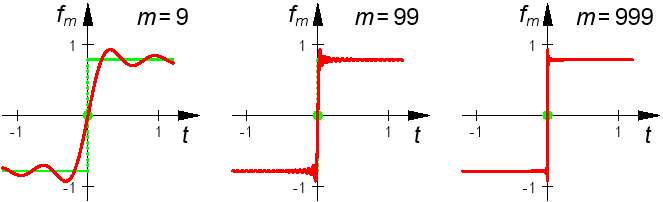
\includegraphics[width=8cm]{./bilder/gibssches_phaenomen.png}  
  \end{minipage}
\end{figure}

Bei Unstetigkeitsstellen konvergiert die Fourierreihe gegen:\\
$\frac{f(t_0-0)+f(t_0+0)}{2}$

\skriptsubsection{Frequenz-, Amplituden- und Phasengang}{72}
$ \text{Frequenzgang eines Systems: } H(\omega) = A(\omega) \cdot e^{j \Phi(\omega)} \qquad 
\text{ Amplitudengang: } A(\omega) = |H(\omega)| \qquad \text{ Phasengang } \Phi(\omega) = arg[H(\omega)] $ \\ \\
Die komplexe Funktion $H(\omega)$ der reellwertigen Frequenz $\omega$ enthält zugleich die Informationen über 
die Veränderung der Amplitude und der Phasenverschiebung des Systems S bei der betrachteten Frequenz $\omega$.
$$f(t) = Im[z(t)] \to \fbox{S}\to F(t) = Im[z(t) \cdot H(\omega)] \qquad \text{ oder } 
\qquad f(t) = Re[z(t)] \to \fbox{S}\to F(t) = Re[z(t) \cdot H(\omega)]$$
Je nach Eingangssignal wird der Real- oder der Imaginärteil behandelt: 
$ f(t) = 
    \left\{
    \begin{array}{l}
           sin(n t) = Im[e^{j \cdot n t}]\\
           cos(n t) = Re[e^{j \cdot n t}]
        \end{array}
    \right\}
\Longrightarrow
z(t) = e^{j \cdot n t}
$ \\

Somit kann die Antwort des Systems mittels einer komplexen Multiplikation mit der Hilfsfunktion $z(t)$ berechnet werden.
